\documentclass{article}
\usepackage{iclr2027_conference,times}

\usepackage{amsmath,amssymb,amsthm}
\usepackage{booktabs}
\usepackage{graphicx}
\usepackage{microtype}
\usepackage{algorithm}
\usepackage{algpseudocode}
\usepackage[utf8]{inputenc}
\usepackage{url}
\usepackage{hyperref}

\graphicspath{{figures/}}

\newtheorem{proposition}{Proposition}
\newtheorem{definition}{Definition}
\newtheorem{assumption}{Assumption}
\newcommand{\spg}{\mathrm{spg}_\tau}

\title{A Measured Identifiability Ceiling for Rendered Scientific Images,\\
and What It Attributes}

% Authors are hidden while \iclrfinalcopy is commented out; the style file
% typesets "Anonymous authors / Paper under double-blind review" in its place.
\author{Anonymous}

%\iclrfinalcopy % Uncomment for the camera-ready version, but NOT for submission.

\begin{document}
\maketitle

\begin{abstract}
\input{sections/00_abstract}
\end{abstract}

\section{Introduction}
A model that misreads a scientific figure and a model that misreasons about it produce the same wrong
answer. Separating the two requires knowing what the figure contains, and for natural images that quantity
does not exist: there is no procedure that reads a photograph's information content without a model.

Rendered scientific figures are different. A ball-and-stick crystal render is an orthographic projection of
a structure whose atomic coordinates are known exactly, under a camera set the experimenter chose. The
projection is invertible in a sense we make precise in Section~\ref{sec:oracle}: given the render's own
geometry, atom positions can be recovered by triangulating across views, and a deterministic symmetry
algorithm applied to the reconstruction returns the answer the images support without consulting a model at
any step. This paper builds that instrument and reports what it attributes.

The shape of the argument has prior art. \citet{arc2512} argue that the gap on abstract-reasoning
benchmarks reflects visual perception rather than inductive reasoning, and verify it with a two-stage
pipeline that converts each image to a natural-language description before inducing rules.
\citet{xcrys2506} reach a compatible conclusion for crystallographic images, and \citet{allangles2504} show
that multi-view geometric correspondence is a known weakness. What differs here is the exactness of the
separation. In every prior design we found, the perception stage is itself a model, so the split compares
two model configurations and inherits the describer's errors, and no quantity in the design states how much
of the task is answerable from the image at all. Our separation is deterministic and closed-form, and it
returns a number.

Three contributions follow.
\textbf{(i) A certified-label benchmark with a measured identifiability ceiling.} Labels are computed by a
symmetry algorithm from the source structures rather than annotated, and the evaluation split excludes
every chemical composition present in training, following \citet{xcrys2506}. The ceiling is 0.9524 rather
than 1.0: the render protocol withholds a measurable amount of what the structure contains, so the gap
between the ceiling and a model is separable from the gap between the ceiling and the label
(Proposition~\ref{prop:ident} characterises exactly when the two coincide).
\textbf{(ii) A four-rung attribution ladder.} Each rung removes one capability on the same named
structures, all comparisons paired (Definition~\ref{def:ladder}). Its outcome contradicts the
perception-bottleneck reading it was built to test: with exact geometry supplied as text, the symbolic
residual is the larger deficit for 12 of 14 scored models, and the perception share tracks model strength.
\textbf{(iii) A render-convention intervention, one leg conclusive and one inconclusive.} Two of the frozen
protocol's geometric choices are measurably information-suboptimal by the oracle. A 70-structure model
probe detected no corresponding change, but its discordance rates leave 7 of 16 paired comparisons unable
to detect one at any outcome, so the model leg is \emph{inconclusive rather than null} and is reported as
such.

\section{Related work}
\textbf{Perception versus reasoning in multimodal models.} The claim that multimodal failures are
perceptual rather than inferential is argued in several places. \citet{arc2512} isolate a perception
bottleneck on abstract-reasoning benchmarks via image-to-description conversion. \citet{decouple2605}
decouple the two stages in post-training and find perception the profitable target; \citet{vab2607}
characterise visual access boundaries directly; \citet{dual2509} report that additional reasoning can
\emph{reduce} accuracy, as does \citet{cotdeg2604} for spatial tasks. Our ladder agrees that perception
matters and disagrees about its share: with exact geometry supplied, the symbolic residual is the larger
deficit for 12 of 14 scored models, and the split tracks model strength. The difference is one of
measurement: every prior separation we found substitutes a model for the perception stage, so it cannot
state what the image contains, whereas the oracle rung can.

\textbf{Crystallography with vision--language models.} \citet{xcrys2506} is the closest neighbour: it
stress-tests nine VLMs on rendered crystal structures under spatial- and composition-exclusion protocols.
We adopt its composition-exclusion discipline and its CIF-supplied condition, citing both as prior use
rather than contribution. \citet{xrdbench2605} benchmark VLMs on XRD peak indexing and already establish
that models fail on rendered crystallographic images, which demotes our own difficulty finding to added
vendor breadth on a deterministic-label target. On the model-free side, \citet{cryspnet2003} and
\citet{extinction2411} predict symmetry from composition and from diffraction-consistent descriptors
respectively; both take the opposite input to ours, so neither is comparable to our cell-metric reference.

\textbf{Resolution and render protocol.} \citet{resbench2510} and \citet{nativevis2506} show that dynamic
resolution input is a live failure mode, which is why our protocol is frozen at a single resolution and why
the effective-resolution audit is reported as a render-design observation rather than a finding.
Multi-view correspondence is a documented weakness \citep{allangles2504}, and view selection has been
optimised end-to-end through a differentiable renderer \citep{mvtn2011}, so we claim no novelty for
optimising a render protocol. Our contribution on that axis is that two of the frozen protocol's choices
are measurably information-suboptimal by the oracle, and that an underpowered model probe detected no
corresponding change.

\textbf{Verifying intermediate steps.} \citet{groundscore2603} verify explicit visual premises to make
process reward models reliable, and \citet{cvt2511} add continuous visual tokens to improve intermediate
visual reasoning. Both share our premise that the intermediate must be checkable. The difference is that a
crystal render admits an exact check against ground-truth coordinates, which is what exposes the
fabrication in Section~\ref{sec:ladder}.

\input{sections/03_setup}
\section{Benchmark construction}
\label{sec:benchmark}

\textbf{Certified labels.} Each structure's crystal system, Bravais lattice, point group and space group
are derived from its coordinates by $\spg$ at the canonical tolerance, with a tolerance sweep that
quarantines any structure whose space group is not stable across it. On the kept set, label agreement with
the source databases is $220/220$ (one-sided exact 95\% lower bound $0.9865$).

\textbf{Composition exclusion.} No chemical composition in any evaluation set appears in training. Without
this, symmetry is partly predictable from composition alone, a published task \citep{cryspnet2003}, and a
model could score well without reading the image.

\textbf{A label ladder gives a difficulty axis.} Figure~\ref{fig:ladder} (right) scores four labels of
increasing granularity for the model-free arms. The oracle is flat across granularity because a
reconstruction is either right or wrong and all four labels follow from it; the cell-metric baseline falls
from 0.8952 at crystal system to 0.6810 at space group, because point group and space group depend on atom
positions that lattice parameters do not encode. The identifiability claim is therefore not specific to the
seven-way label.

\begin{figure}[t]
\centering
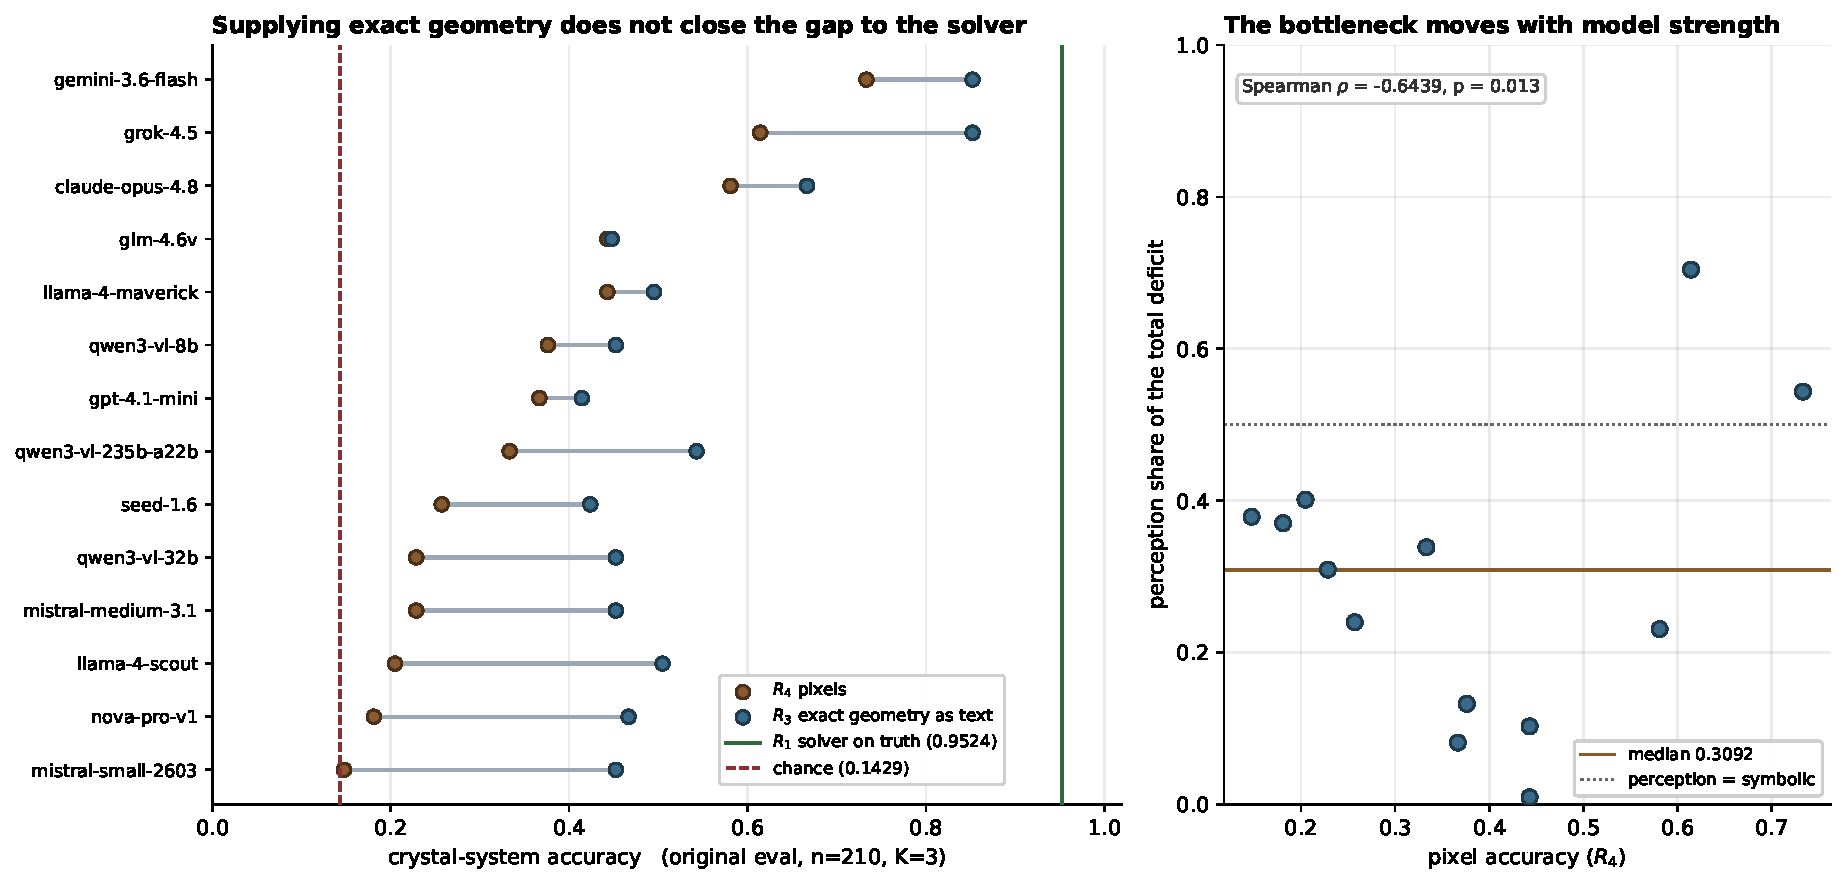
\includegraphics[width=0.8\linewidth]{figures/ladder.pdf}
\caption{Left: attribution ladder, original evaluation sample ($n=210$); rungs as in
Definition~\ref{def:ladder}, $R_2$ omitted (unscored under its pre-registered gate). Right: label ladder
across four label granularities for the model-free arms; the oracle (top curve) is flat, the cell-metric
baseline is not.}
\label{fig:ladder}
\end{figure}

\section{The attribution ladder}
\label{sec:attribution}

\begin{definition}[Rungs and shares]
\label{def:ladder}
For a model $m$ evaluated on the same structures, let
$R_0 = \tfrac{1}{n}\sum \mathbf{1}[\spg(s) = y(s)]$ (the symmetry algorithm on ground-truth positions),
$R_1$ the oracle ceiling of Definition~\ref{def:ceiling},
$R_3(m)$ the accuracy of $m$ given ground-truth fractional coordinates, species and cell parameters as
text, and
$R_4(m)$ the accuracy of $m$ on the pixel renders. Define the \emph{perception component}
$P(m) = R_3(m) - R_4(m)$, the \emph{symbolic residual} $S(m) = R_1 - R_3(m)$, and the \emph{perception
share} $P(m) / (R_1 - R_4(m))$. $R_2$ denotes the oracle run on a learned detector's output.
\end{definition}

Three conditions make the shares interpretable, and we state them because each is checkable: the rungs are
scored on the same named structures with all comparisons paired; $R_3$ and $R_4$ use the same decode budget
($K{=}3$ everywhere the shares are computed); and the symbolic residual \emph{bounds} rather than isolates
symmetry reasoning, since a residual against a deterministic solver can include failure modes other than
symmetry (we test this directly below). Table~\ref{tab:rungs} gives the ladder.

\begin{table}[t]
\centering
\caption{Attribution ladder, original evaluation sample, $n=210$, $K{=}3$. The two model columns are the
strongest scored model and one mid-roster model, named rather than aggregated; $R_3$ and $R_4$ within
a column are the same model under two conditions, so their interval is that model's perception component
(Definition~\ref{def:ladder}). $R_2$ is unscored: its extractor fails to triangulate on 19.0\% and 22.4\%
of structures, over the pre-registered 5\% gate. The fine-tuned arm was never run under the coordinate
condition, so it carries no within-model interval and is not a column.}
\label{tab:rungs}
\small
\setlength{\tabcolsep}{4.5pt}
\begin{tabular}{p{0.40\linewidth}p{0.22\linewidth}rr}
\toprule
rung & what it removes & \small gemini-3.6-flash & \small gpt-4.1-mini \\
\midrule
$R_0$ algorithm on ground-truth positions & nothing & \multicolumn{2}{c}{1.0000 (definitional)} \\
$R_1$ oracle: camera inversion, then algorithm & the protocol's losses & \multicolumn{2}{c}{0.9524} \\
$R_3$ exact geometry as text ($K{=}3$) & the model's perception & 0.8524 & 0.4143 \\
$R_4$ pixels ($K{=}3$) & nothing further & 0.7333 & 0.3667 \\
\midrule
perception share $(R_3-R_4)/(R_1-R_4)$ & --- & 0.5436 & 0.0813 \\
$R_2$ oracle on a learned detector's output & ideal extraction & \multicolumn{2}{c}{unscored} \\
\bottomrule
\end{tabular}
\end{table}

\textbf{The top rung is definitional, and that is load-bearing.} The label \emph{is} $\spg$ applied to the
structure, so $R_0 = 1.0000$ exactly, and the $R_0 \to R_1$ interval is what camera inversion and
correspondence re-solution cost. Treating $R_0$ as approximately equal to $R_1$ would discard that
interval.

\textbf{Exact geometry does not close the gap.} Supplying ground-truth geometry as text (the CIF-supplied
condition of \citet{xcrys2506}, cited as prior use) lifts every model substantially, and none reaches the
oracle: the best is 0.8524 against 0.9524. The pre-registered decomposition of Definition~\ref{def:ladder}
gives a median perception share of 30.9\% across the 14 models scored under the coordinate condition, with
the symbolic residual the larger of the two for 12 of them; the two columns of Table~\ref{tab:rungs} differ
in perception share by a factor of six. Only the two strongest models are perception-dominated, and the
share tracks pixel accuracy (Spearman $\rho = -0.6439$, $p = 0.0130$). \emph{The bottleneck moves with
model strength}: a more precise statement than either single attribution, and one visible only because the
oracle fixes the top of the ladder.

\textbf{A control pair makes $R_3$ readable.} Removing the images and leaving only the chemical formula
collapses every scored model toward seven-way chance (mean 0.1487 over the 13 models scored under the
image-removal control). Removing the images and supplying full geometry lifts every scored model to
between 0.4143 and 0.8524.
The two conditions differ in one thing, so the lift is the geometry rather than text-mode prompting; the
geometry prompts are also shorter than the five-image prompts they beat, which rules out a length artefact.

\textbf{The symbolic residual is an upper bound, and we tested it.} A residual against a solver may include
long-list handling rather than symmetry reasoning. Regressing per-structure $R_3$ correctness on
conventional-cell atom count over the same records (no new model calls): pooled over the 14 scored models
and 2940 model-structure pairs, Spearman $\rho = -0.0908$ at $p = 8.1\times10^{-7}$; 13 of 14 models are
negative, and accuracy falls from 0.5551 on cells at or below the median 14 atoms to 0.5129 above it
(Fisher $p = 0.0241$). The pre-registered confound control does not rescue it: atom count correlates with
crystal system ($\rho = -0.1866$), but the mean within-system association is $-0.1053$, stronger than the
pooled figure rather than attenuated, so the effect is not symmetry difficulty in disguise. We therefore
report the symbolic residual as an upper bound on a symmetry-reasoning deficit, not as a measurement of
one. Nothing here touches the oracle-to-model gap, which is measured against pixels.

\textbf{A learned extractor fabricates its output.} Substituting a strong model as the extraction stage,
prompted for species and positions with the symmetry question withheld, and having a weaker model answer
from that text yields 0.1429. That arm predicted two of seven classes and its accuracy equals the majority
stratum's base rate, so it measures nothing. The informative measurement is the intermediate, scored
directly against ground truth: median recall 0.0000, with 105 of 206 structures having not one emitted atom
within tolerance of a real one, despite a median of 48 well-formed atoms per structure. A colour-threshold
blob detector achieves median recall 0.400 on the same task. Downstream accuracy alone would have read this
as bad reasoning. \emph{A two-stage pipeline whose intermediate cannot be checked will attribute
fabrication to reasoning}, which is the argument for the instrument.

\begin{figure}[t]
\centering
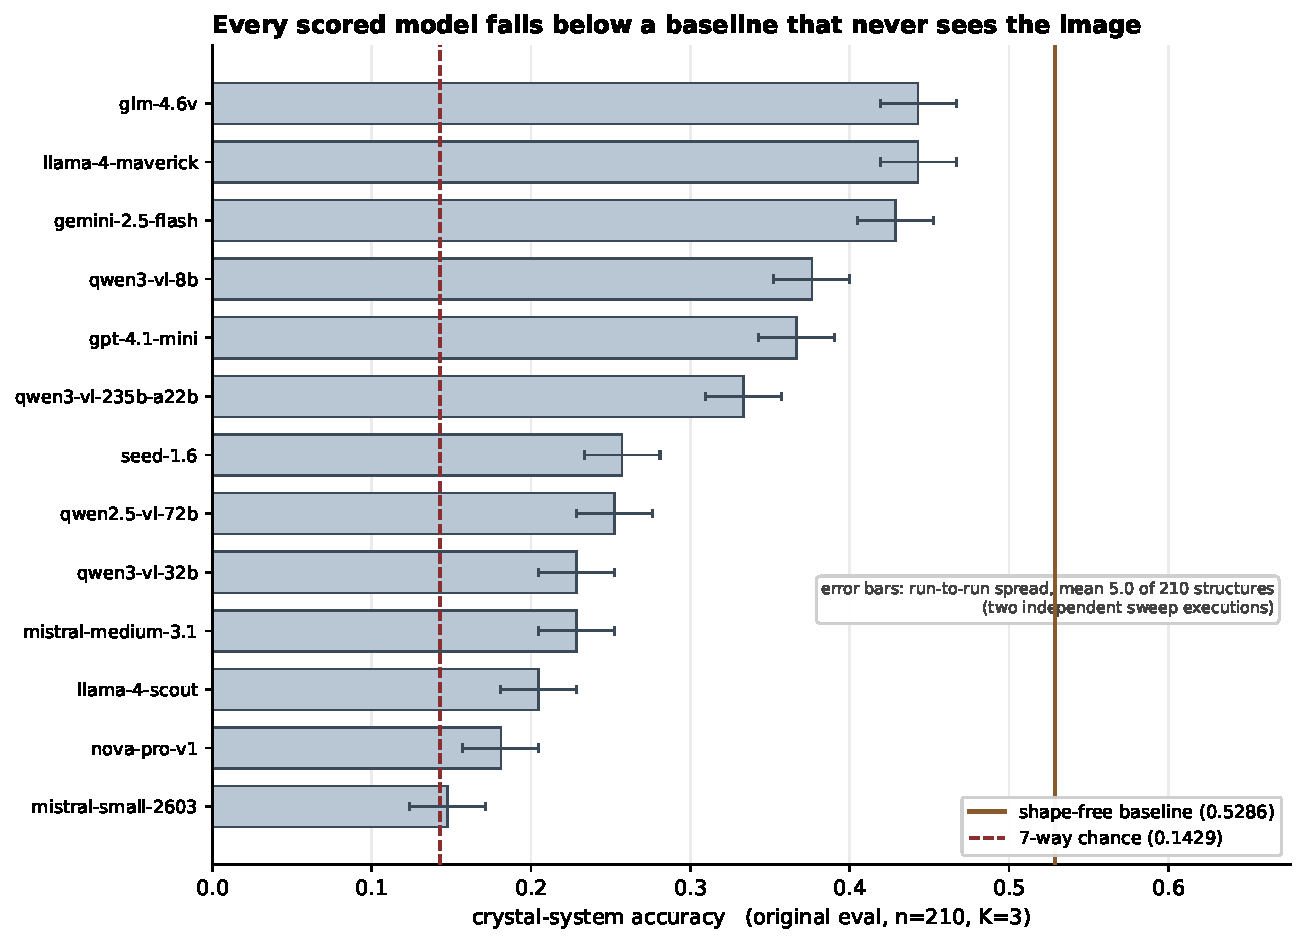
\includegraphics[width=0.8\linewidth]{figures/leaderboard.pdf}
\caption{Zero-shot leaderboard, original sample, $n=210$, $K=3$, 13 scored models across eight vendors.
Dashed line: the shape-free baseline (atom count, density, cell volume) on this sample. Error bars: the
measured run-to-run spread of $K{=}3$ majority voting.}
\label{fig:leaderboard}
\end{figure}

\section{Where models sit}
\label{sec:models}

\textbf{Rosters.} Three conditions were run over overlapping but non-identical model sets, so we name each
roster explicitly and never write a bare count. The zero-shot leaderboard scored 13 of a pre-registered 14,
with \texttt{moonshotai/kimi-k2.6} unscored under an endpoint-failure gate (no response on a two-structure
$K{=}1$ probe after ten minutes, so the failure is the endpoint rather than the harness); it includes
\texttt{google/gemini-2.5-flash} and not the newer \texttt{gemini-3.6-flash} that heads the ladder, which
is why the leaderboard's best row (0.4429) sits below the ladder's best $R_4$ (0.7333). The image-removal
control attempted 16 and scored 13, with three unscored under a pre-registered 5\% API-error gate. The
coordinate condition attempted 15 and scored 14, with \texttt{qwen/qwen2.5-vl-72b-instruct} unscored for
exceeding both the error and parse gates (34.4\% errors). Every unscored entry is reported unscored rather
than dropped; the per-model roster table is in the supplementary.

The 13 scored zero-shot models ran on the frozen protocol with a verbatim prompt and no per-model tuning
(Figure~\ref{fig:leaderboard}). The best reaches $93/210 = 0.4429$ on the original sample, far below the
oracle's 0.9524.

\textbf{A baseline comparison we previously reported does not survive scale-up, and we retire it.} On the
original sample every model falls below a shape-free baseline reading only atom count, density and cell
volume (0.4429 against 0.5286, one-sided $p = 0.0078$). We regenerated the evaluation set at $n = 1933$
under identical rules: same composition exclusion, verified zero overlap with training and both earlier
samples, stratified 285 per system before quarantine, with 62 structures (3.11\%) removed for label
instability under the tolerance sweep. On that sample the baseline falls to 0.2054. Because the new draw
also has larger cells (median 38 atoms against 14), we ran a size-matched control restricted to the
original's 95th percentile: the baseline is 0.2205 there, so the shift is not a cell-size artefact.
\emph{The 0.5286 was a property of the original draw, not of the task}, and the below-baseline claim is
scoped to that sample rather than asserted generally.

The same control shows the oracle's apparent drop at scale \emph{is} a cell-size effect: 0.8774 on the full
sample but 0.9459 at matched cell size, within 0.0065 of the original. More atoms per cell means more
projective coincidence and more correspondence ambiguity, which is the failure set of
Proposition~\ref{prop:ident}. The ceiling-to-model gap, which is what this paper rests on, therefore
survives scale-up (0.9459 against 0.4429), while the baseline comparison does not.

\textbf{Run-to-run spread is a benchmark property.} An unplanned second execution of the sweep gives a mean
absolute difference of 5.0 structures and a maximum of 11, so adjacent leaderboard rows are not separable
and the ordering is not exact.

\textbf{A modality-matched reference.} A cell-metric random forest reaches 0.8952 on crystal system, above
every model. This reproduces an established capability rather than contributing one; it is not comparable
to \citet{cryspnet2003}, which predicts symmetry from composition alone, the opposite input and a harder
problem.

\textbf{The models do use the image.} A benchmark on which models score poorly invites the objection that
they are pattern-matching the prompt rather than reading the figure. We ran the image-absent control that
\citet{cotdeg2604} made standard: the identical prompt carrying the chemical formula and no renders. Every
scored model collapses toward seven-way chance (mean 0.1487), and the paired per-structure difference is
significant for 10 of the 13 models scored under the image-removal control (Figure~\ref{fig:noimage}); the
strongest model loses 0.5714. The three nulls are the three weakest models, two of which are not above
chance even with images, so those are floor effects rather than evidence of formula lookup.

\begin{figure}[t]
\centering
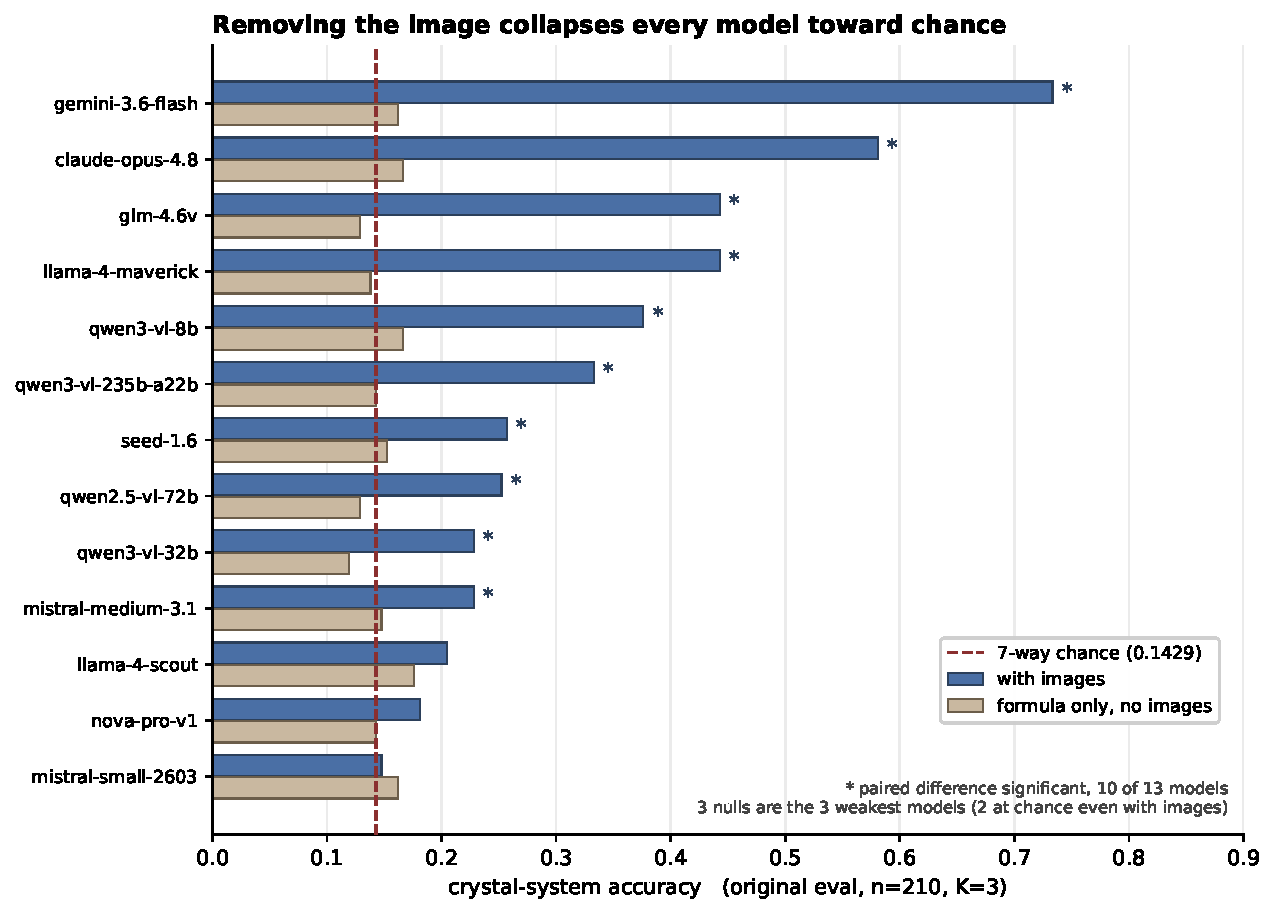
\includegraphics[width=0.8\linewidth]{figures/noimage.pdf}
\caption{Image-removal control: each model answered the identical prompt with the five renders and with the
chemical formula alone, paired per structure (original sample, $n=210$, $K=3$, 13 scored of 16 attempted).
Stars mark models whose paired difference is significant; the dashed line is seven-way chance.}
\label{fig:noimage}
\end{figure}

\paragraph{The strongest model arm, and what is not claimed for it.}
The 0.6905 figure is a supervised-then-GRPO arm on \texttt{Qwen/Qwen3-VL-8B-Instruct}, reported as a
single-seed point estimate at $K{=}8$; the same adapter gives $139/210 = 0.6619$ at $K{=}3$. It sits inside
the reference arm's across-seed spread ($0.590 / 0.567 / 0.686$), exceeding that arm's best seed by one
structure at $K{=}8$ and trailing it by five at $K{=}3$, so \emph{we make no claim that this arm improves
on the reference arm}. It is used only as the model side of the ceiling-to-model gap (200 against 145,
discordance $61{:}6$, $p = 1.5\times10^{-12}$), which survives any seed in the observed spread. The
three-seed extension was cut; its record and the quantitative argument for the cut are in the
supplementary.

\input{sections/07_conventions}
\section{Secondary analyses}
\label{sec:secondary}

Two axes are reported in full in the supplementary and summarised here, because both end by disclaiming
themselves and neither carries a main-text claim.

\textbf{Cue sufficiency.} Whether the conventional-cell metric alone determines the crystal system splits
the samples $140/70$ and $141/69$ and is a stable property of the render convention with no accuracy
mechanism attached: an earlier claim that pixel accuracy simply drops on the ambiguous stratum failed four
independent tests and is withdrawn. A contrast against a cell-metric control does widen on that stratum for
all three frontier models on both samples (Figure~\ref{fig:cuesuff}), but the stratum is $60/70$ and
$58/69$ hexagonal-or-trigonal, so the finding is close to a restatement of that one degeneracy, and the
degeneracy-removed residual rests on $n=10$ and $n=12$.

\textbf{One generation of model progress.} It does not erase the axis (Figure~\ref{fig:generational}): from
gemini-2.5-flash to gemini-3.6-flash the newer model gains more on the ambiguous stratum in raw terms but
closes less of its headroom to the oracle (54.1\% against 64.0\%), and one model pair is a comparison
rather than a trend.

\section{Limitations}
\textbf{No human baseline.} Recruitment of qualified crystallographers failed. We therefore make no claim
that the renders are solvable by humans; the oracle stands in for the information question only, and
``adequate'' means recoverable by a geometric reader.

\textbf{What the oracle does not license.} It reads ground-truth coordinates, not pixels. It bounds what is
recoverable given ideal extraction and says nothing about achievable extraction. The extraction share of
the ceiling-to-model gap is bounded from neither side: $R_1$ assumes perfect extraction and $R_2$'s
extractor is too weak to be informative. A detector at recall above 0.9 is the most valuable missing
measurement.

\textbf{Sample size.} All model numbers rest on two samples of 210; the minimum detectable paired
difference there is near 0.09, so adjacent leaderboard rows are not separable. The model arms were not
re-run at $n = 1933$ (that is $19{,}500$ calls on a 500-structure core), so the ceiling-to-model gap at
scale is bounded on the oracle side only. The oracle and both classical baselines are complete on the full
1933.

\textbf{Corrections and non-recoveries.} Three published values did not reproduce from their own records
and are documented as non-recoveries rather than silently replaced: an earlier cue-sufficiency classifier's
exact rule, an oracle view-count curve, and the tabular classifier's published count (twelve defensible
readings of its recorded protocol span 183 to 188 without reaching the published 186). A previously
published minimum-detectable-difference for the render-convention null was computed with an unpaired
approximation and is retracted in favour of the per-comparison analysis of Section~\ref{sec:conventions},
which makes that null weaker rather than stronger. The full retraction ledger is in the supplementary
(Appendix~\ref{app:corrections} indexes it).

\input{sections/10_conclusion}

% Reproducibility and AI-use statements: unnumbered, excluded from the page limit.
\input{sections/11_statements}

\bibliographystyle{iclr2027_conference}
\bibliography{references}

\appendix
\section{Proof sketch for Proposition~\ref{prop:ident}}
\label{app:proof}
Let atom $a$ have Cartesian position $p \in \mathbb{R}^3$ and let $v, w$ be two views with linearly
independent directions $d_v, d_w$. Its images are $q = P_v p$ and $q' = P_w p$. The back-projections are
the affine lines $\ell_v = \{x : P_v x = q\}$ (direction $d_v$) and $\ell_w = \{x : P_w x = q'\}$
(direction $d_w$). Both contain $p$; since $d_v \not\parallel d_w$, two non-parallel lines in
$\mathbb{R}^3$ that intersect do so in exactly one point, so $\ell_v \cap \ell_w = \{p\}$ and the
intersection step of Algorithm~\ref{alg:oracle} recovers $p$ exactly from the correct pairing. It remains
to show no incorrect pairing survives. A spurious pairing $(q, q'')$ with $q''$ the image of a different
atom $b$ either yields no intersection (skew lines, rejected) or yields a point $\hat{p} \neq p$ whose
projections must, by hypothesis (ii), fall outside the matching tolerance of any same-species point in at
least one remaining view, so the verification step rejects it. The verified reconstruction is
therefore exactly the atom set, on which $\spg$ returns $y(s)$ by the definition of the label.
Condition (ii) is where the argument is not vacuous: it fails precisely on projective coincidence, when
distinct atoms project within tolerance of one another in the verifying views. The measured ceiling gap
(0.0476 on the original sample) and its growth with atoms per cell (Section~\ref{sec:models}) are
measurements of that failure set.

\section{Statistical procedures}
\label{app:stats}
\textbf{Paired comparisons.} Every model-versus-model and model-versus-oracle comparison on a shared sample
is a paired exact binomial (sign) test on discordant structures: with $g$ structures one arm alone gets
right and $l$ the other alone, the two-sided $p$ is that of $\mathrm{Bin}(g+l, 1/2)$ evaluated at
$\min(g,l)$. For the render-convention probe, the per-comparison minimum detectable difference is the
smallest $|g-l|/n$ reaching $p<0.05$ given that comparison's observed $g+l$; with $g+l \le 5$ no split
reaches it, which is the source of the 7-of-16 unreachable comparisons in
Section~\ref{sec:conventions}.
\textbf{Label certification.} The one-sided exact 95\% lower bound for $k/k$ agreements is
$0.05^{1/k}$; for $k = 220$ this is $0.9865$.
\textbf{Run-to-run spread.} The second sweep execution is retained as a labelled replication; spread is
reported as the mean and maximum absolute per-model difference in correct counts.

\section{Index of corrections and non-recoveries}
\label{app:corrections}
The full retraction ledger, verbatim and in checkpoint order, is in the supplementary. Main-text items:
the retired below-baseline claim (Section~\ref{sec:controls}), the retracted unpaired
minimum-detectable-difference (Section~\ref{sec:conventions}), the withdrawn stratified-accuracy mechanism
(Section~\ref{sec:controls}), and the three documented non-recoveries (Limitations). 
\section{Supporting figures}
\label{app:secondary}
The visibility-conditioned oracle of Section~\ref{sec:conventions} and the two secondary axes of
Section~\ref{sec:controls} are stated numerically in the main text; their figures are placed here.

\begin{figure}[htbp]
\centering
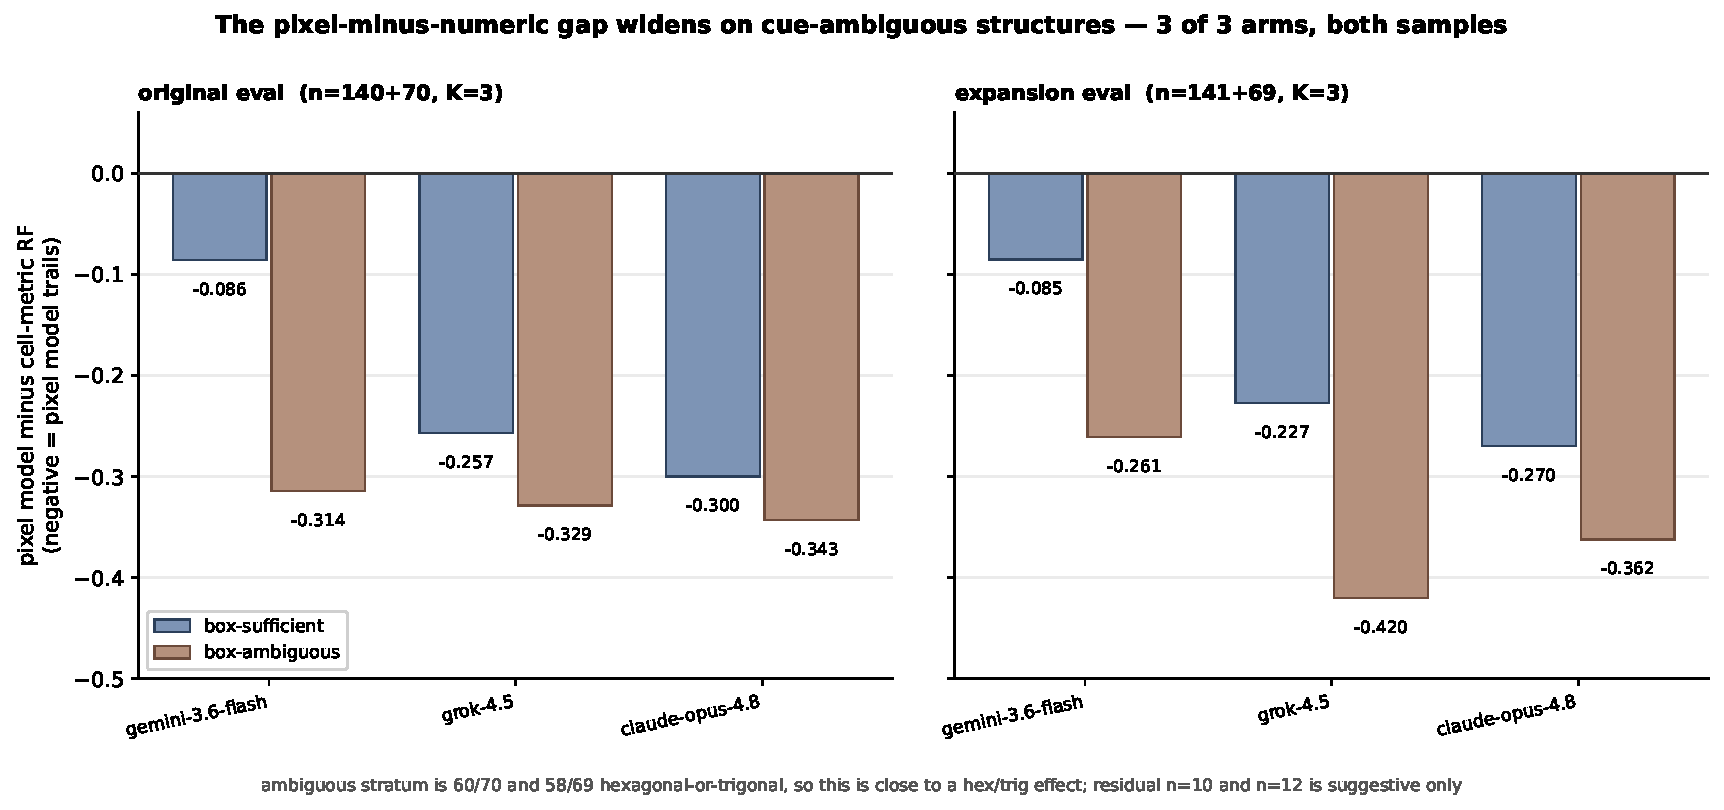
\includegraphics[width=0.8\linewidth]{figures/cuesuff.pdf}
\caption{Pixel accuracy minus a cell-metric random forest on the same structures, by cue-sufficiency
stratum, three frontier models, both evaluation samples ($K=3$). Negative means the pixel model trails the
numeric reader. Stratum composition is annotated on the panels; see Section~\ref{sec:controls}.}
\label{fig:cuesuff}
\end{figure}

\begin{figure}[htbp]
\centering
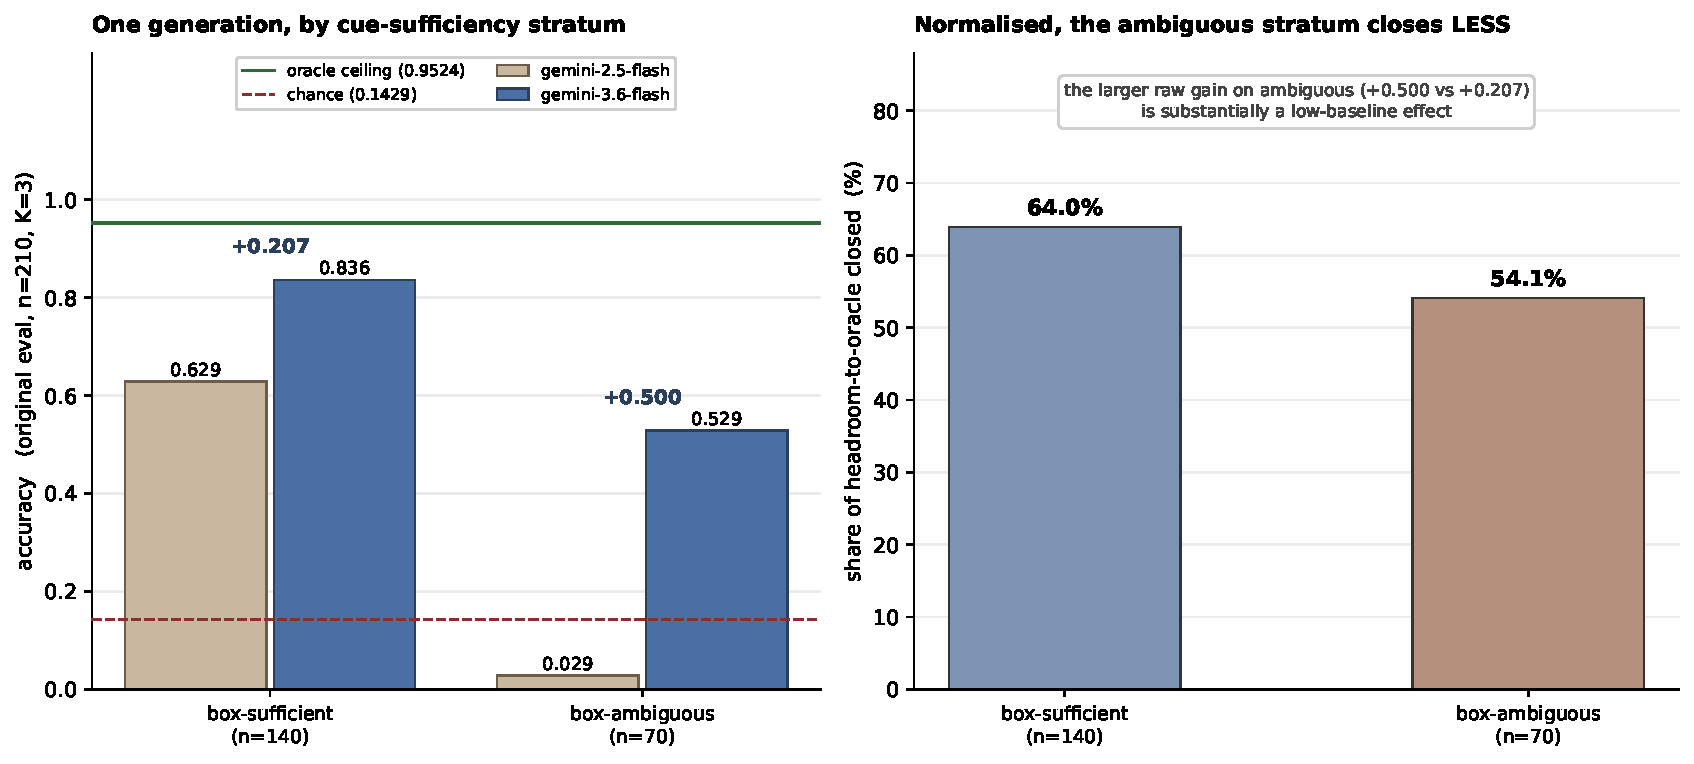
\includegraphics[width=0.8\linewidth]{figures/generational.pdf}
\caption{One generation of model progress, original sample, $n=210$, $K=3$. Left: raw accuracy by
cue-sufficiency stratum, with the oracle ceiling and seven-way chance drawn. Right: the same gains
normalised by headroom to the oracle.}
\label{fig:generational}
\end{figure}

\begin{figure}[htbp]
\centering
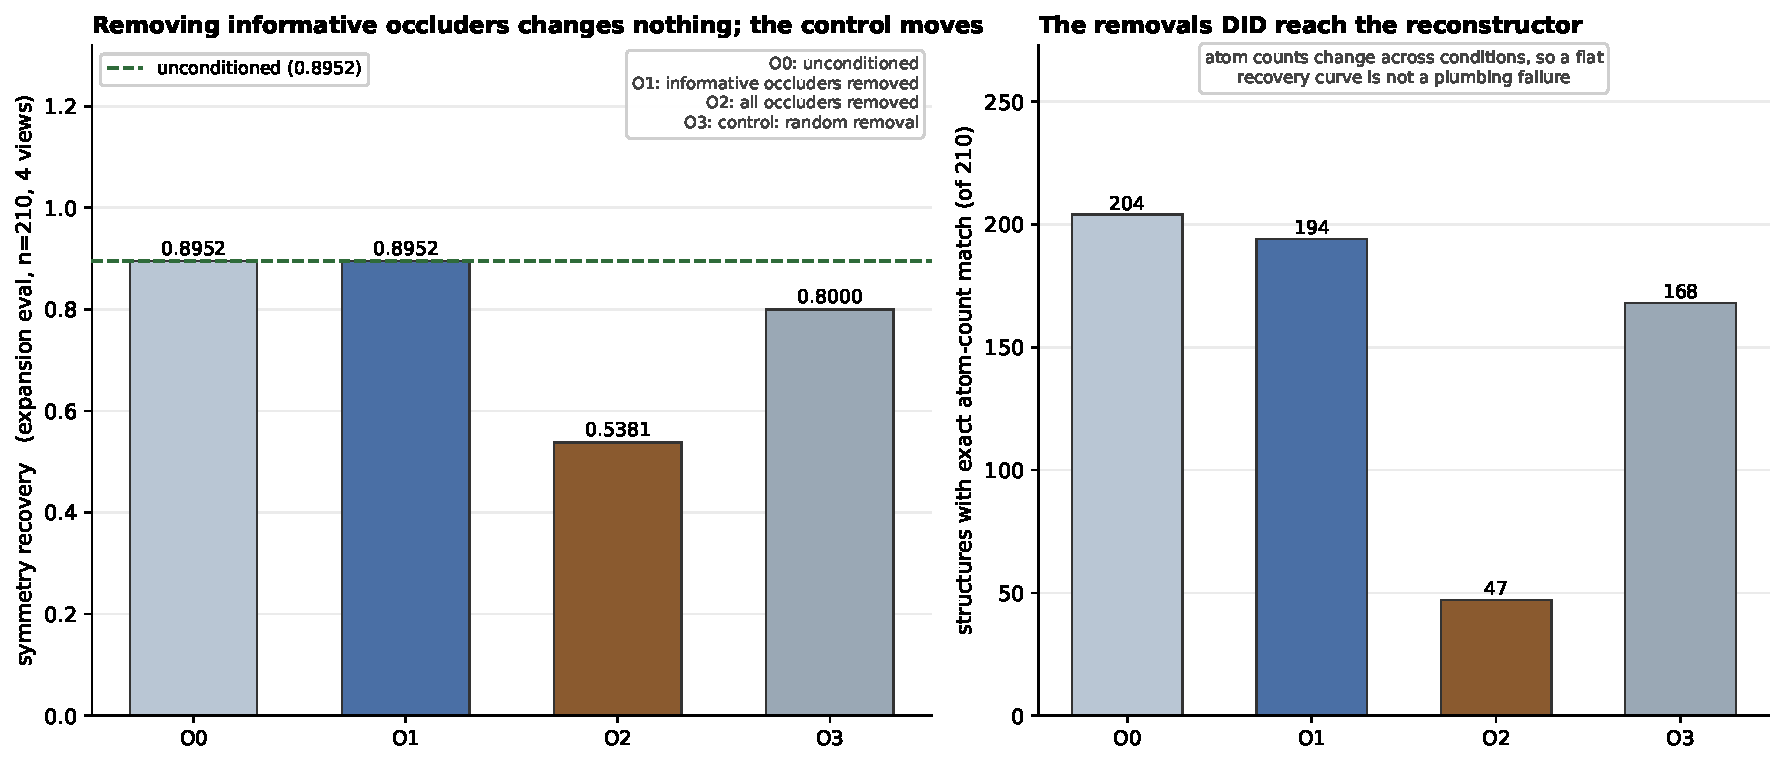
\includegraphics[width=0.8\linewidth]{figures/conditions.pdf}
\caption{Visibility-conditioned oracle: recovery when informative occlusion is removed from the oracle's
input, when redundant occlusion only is removed (pre-registered control), and unconditioned, on both
evaluation samples.}
\label{fig:conditions}
\end{figure}


\end{document}
